% ===========================================================================
\section{Milestone I: The background cosmology}\label{sec:m1}
% ===========================================================================

The first milestone computes the expansion history of a homogeneous and isotropic Universe. Every later module
needs it: the recombination rates are set by the competition between atomic reaction rates and the expansion rate
$H$, the perturbation equations contain $\Hp$ and its derivatives, and the line-of-sight integral needs the conformal
distance $\eta_0-\eta$ to the last-scattering surface. The background also contains the first test of the model
against data, through the distances to type Ia supernovae.

\subsection{Theory}

\paragraph*{The metric and the Friedmann equations.} The cosmological principle states that on large scales the
Universe is homogeneous and isotropic. The most general metric with these symmetries is the
Friedmann--Lema\^itre--Robertson--Walker (FLRW) metric,
\begin{equation}
\dd s^2 = -c^2\dd t^2 + a^2(t)\Big[\frac{\dd r^2}{1-kr^2} + r^2\dd\Omega^2\Big],
\end{equation}
where $r$ is a comoving radial coordinate, $k$ is the spatial curvature and $a(t)$, normalized to $a(t_0)=1$ today,
is the scale factor. All the dynamics is in $a(t)$. Because of the symmetry, the matter content must be a set of
perfect fluids with energy density $\rho_i c^2$ and pressure $P_i=w_i\rho_ic^2$. Inserting the metric and fluids in
Einstein's equations gives two independent equations. The $00$ component is the Friedmann equation,
\begin{equation}
H^2\equiv\Big(\frac{\dot a}{a}\Big)^2 = \frac{8\pi G}{3}\sum_i\rho_i - \frac{kc^2}{a^2},
\label{eq:friedmann}
\end{equation}
and the trace of the $ij$ components gives the acceleration equation,
\begin{equation}
\frac{\ddot a}{a} = -\frac{4\pi G}{3}\sum_i\Big(\rho_i+\frac{3P_i}{c^2}\Big).
\label{eq:accel}
\end{equation}
Combining them gives energy conservation, $\dot\rho_i+3H(\rho_i+P_i/c^2)=0$, which for constant $w_i$ integrates to
$\rho_i\propto a^{-3(1+w_i)}$. The relevant cases are:
\begin{itemize}
\item Non-relativistic matter (baryons and cold dark matter), $w=0$. The number of particles in a comoving volume is
      conserved, so $\rho_M\propto a^{-3}$.
\item Radiation (photons and massless neutrinos), $w=1/3$. The number density falls as $a^{-3}$ and, in addition, every
      particle loses energy to the redshift, $E\propto a^{-1}$, so $\rho_r\propto a^{-4}$.
\item A cosmological constant, $w=-1$, with $\rho_\Lambda$ constant: the vacuum energy per volume does not dilute.
\end{itemize}
Curvature enters Eq.~\eqref{eq:friedmann} like a fluid with $\rho\propto a^{-2}$. Dividing by $H_0^2$ and defining
the density parameters relative to the critical density $\rho_{c0}=3H_0^2/8\pi G$ (the density of a flat universe),
$\Om_{i0}=\rho_{i0}/\rho_{c0}$ and $\Om_{K0}=-kc^2/H_0^2$, gives
\begin{equation}
H(x) = H_0\sqrt{\Om_{M0}e^{-3x} + \Om_{r0}e^{-4x} + \Om_{K0}e^{-2x} + \Om_{\Lambda0}} ,
\label{eq:H}
\end{equation}
where $\Om_M=\Om_b+\Om_{\rm CDM}$ and $\Om_r=\Om_\gamma+\Om_\nu$. We use $x=\ln a$ as time variable. The interesting
history spans some twenty $e$-folds of expansion, and most quantities vary as powers of $a$, which are simple
exponentials in $x$. Evaluating Eq.~\eqref{eq:H} today gives the constraint $\sum_i\Om_{i0}=1$, which fixes
$\Om_{\Lambda0}$ in a flat universe. The density parameters at other times are
$\Om_i(x)=\Om_{i0}e^{-n_ix}H_0^2/H^2(x)$, with $n_i=3,4,2,0$ for matter, radiation, curvature and $\Lambda$; they
measure which component drives the expansion at a given time.

\paragraph*{The radiation density.} The CMB is a blackbody with temperature $T_{\rm CMB}=2.7255$\,K, so its density
follows from the Stefan--Boltzmann law: integrating the Bose--Einstein distribution over momenta, with two
polarization states, gives $\rho_\gamma c^2=2\cdot\frac{\pi^2}{30}(k_BT)^4/(\hbar c)^3$ and
\begin{equation}
\Om_{\gamma0} = 2\cdot\frac{\pi^2}{30}\frac{(k_BT_{\rm CMB})^4}{\hbar^3c^5}\cdot\frac{8\pi G}{3H_0^2}.
\end{equation}
Neutrinos decoupled from the plasma at $T\sim1$\,MeV, just before electrons and positrons annihilated. The annihilation
heated the photons but not the neutrinos, and entropy conservation gives $T_\nu=(4/11)^{1/3}T_\gamma$ afterwards.
Fermions also carry a factor $7/8$ relative to bosons in the energy density. With $N_{\rm eff}$ species,
$\Om_{\nu0}=N_{\rm eff}\,\tfrac{7}{8}(4/11)^{4/3}\Om_{\gamma0}$. $N_{\rm eff}=3.046$ rather than 3 because the
neutrinos were still slightly coupled when the annihilation began and shared a little of its energy.

\paragraph*{Clocks and horizons.} Cosmic time $t$ is the time measured by an observer at rest with respect to the
expansion. Conformal time $\eta$ is defined by $c\,\dd t=a\,\dd\eta$, so that light moves on straight lines in
$(\eta,\chi)$ coordinates with $\dd\chi=c\,\dd\eta$. In terms of $x$,
\begin{equation}
\frac{\dd t}{\dd x} = \frac{1}{H}, \qquad \frac{\dd\eta}{\dd x} = \frac{c}{\Hp},\qquad \Hp\equiv aH=\dot a.
\label{eq:eta}
\end{equation}
$\eta(x)$ is the comoving distance light has travelled since the Big Bang, the \emph{particle horizon}. Two regions
farther apart than $\eta$ have never been in causal contact. The quantity $c/\Hp$ is the comoving Hubble radius, the
distance over which the expansion velocity reaches $c$, and over which causal physics can act within one expansion
time. A perturbation of comoving wavenumber $k$ is outside the horizon when $ck<\Hp$ and inside when $ck>\Hp$. In a
decelerating universe ($\ddot a<0$) $\Hp=\dot a$ decreases, so ever larger scales enter the horizon. This is central
for the perturbations of Milestone~III.

\paragraph*{Single-component limits.} If one component with $\rho\propto a^{-n}$ dominates, then
$\Hp\propto a^{1-n/2}=e^{-(n-2)x/2}$, and Eq.~\eqref{eq:eta} gives $\eta=2c/[(n-2)\Hp]$ for $n>2$. Hence
\begin{equation}
\frac{\Hp'}{\Hp}=1-\frac{n}{2},\qquad \frac{\Hp''}{\Hp}=\Big(1-\frac{n}{2}\Big)^2,\qquad \frac{\eta\Hp}{c}=\frac{2}{n-2},
\label{eq:Hp_limits}
\end{equation}
that is $(-1,1,1)$ in radiation domination (RD) and $(-\tfrac12,\tfrac14,2)$ in matter domination (MD). In $\Lambda$
domination $H$ is constant, $\Hp\propto a$, $\Hp'/\Hp=\Hp''/\Hp=1$, and $\eta$ approaches a finite value: there is an
event horizon, and we will never see beyond it. The corresponding laws for cosmic time are $t\propto a^2$ (RD),
$t\propto a^{3/2}$ (MD) and $t\propto\ln a$ ($\Lambda$). These limits are our main tests.

\paragraph*{Distances.} Light from an object at $x$ has travelled a comoving distance $\chi=\eta_0-\eta(x)$. In a
curved universe the comoving \emph{transverse} distance is $r=\chi\,\mathrm{sinn}(\sqrt{|\Om_{K0}|}H_0\chi/c)/
(\sqrt{|\Om_{K0}|}H_0\chi/c)$, with $\mathrm{sinn}=\sinh$ for $\Om_{K0}>0$ and $\sin$ for $\Om_{K0}<0$; for flat space
$r=\chi$. An object of physical size $D$ at scale factor $a$ subtends the angle $\theta=D/(ar)$, so the angular
diameter distance is $d_A=ar$. A source of luminosity $L$ spreads its light over a sphere of comoving area $4\pi r^2$,
and each photon arrives with its energy reduced by $(1+z)$ and its arrival rate reduced by another $(1+z)$ because of
time dilation. The flux is then $F=L/(4\pi d_L^2)$ with the luminosity distance $d_L=r/a=(1+z)^2d_A$.

At low redshift $d_L\simeq cz/H_0$, Hubble's law. The next term,
$d_L\simeq(cz/H_0)[1+\tfrac12(1-q_0)z]$, depends on the deceleration parameter $q_0=-\ddot a/(aH^2)|_0=
\tfrac12\Om_{M0}-\Om_{\Lambda0}$ (neglecting radiation). In an accelerating universe ($q_0<0$) distant objects are
farther away, and therefore fainter, than in a decelerating one. This is how supernovae revealed the accelerated
expansion.

\paragraph*{Key epochs.} Three epochs are of special interest:
\begin{itemize}
\item Radiation--matter equality, $\rho_r=\rho_M$, at $a_{\rm eq}=\Om_{r0}/\Om_{M0}$.
\item Matter--$\Lambda$ equality at $a^3=\Om_{M0}/\Om_{\Lambda0}$.
\item The onset of acceleration, $\ddot a=0$. Equation~\eqref{eq:accel} shows that a component accelerates the
      expansion only if $w<-1/3$. Matter contributes $\rho_M$ and $\Lambda$ contributes $\rho_\Lambda+3P_\Lambda/c^2=
      -2\rho_\Lambda$, so acceleration starts when $\rho_M=2\rho_\Lambda$, i.e.\ $\Om_{M0}a^{-3}=2\Om_{\Lambda0}$.
      Since $\ddot a=\dot\Hp$, this is also where $\Hp'=0$.
\end{itemize}
The wavenumber that enters the horizon at equality, $k_{\rm eq}=\Hp(x_{\rm eq})/c$, separates modes that entered
during RD from those that entered during MD. It sets the turnover scale of $P(k)$ (Sec.~\ref{sec:m4}).

\subsection{Implementation and tests}

\texttt{BackgroundCosmology} writes $E^2=H^2/H_0^2$ as a sum of virtual component densities, each with analytic first
and second $x$-derivatives. $\Hp$, $\Hp'$ and $\Hp''$ are therefore analytic. A new model, for example dynamical dark
energy, only overrides the density of one component; the code includes a CPL $w_0w_a$ example. We solve
Eq.~\eqref{eq:eta} on $x\in[-20,5]$ with an adaptive Runge--Kutta (RK8PD) solver and store $\eta$ and $t$ in cubic
splines. The initial values come from the exact solution for a universe with radiation and matter only,
\begin{equation}
\eta = \frac{2ca}{H_0\big(\sqrt{\Om_{r0}+\Om_{M0}a}+\sqrt{\Om_{r0}}\big)},
\end{equation}
which is exact up to the negligible $\Lambda$ term at $x=-20$; the analogous expression is used for $t$. The epochs
are found by root finding on the analytic expressions.

Figure~\ref{fig:Hp_tests} shows the two standard tests. $\Hp'/\Hp$ and $\Hp''/\Hp$ reach the plateaus of
Eq.~\eqref{eq:Hp_limits} in each era, with smooth transitions at the equality epochs. $\eta\Hp/c$ goes from 1 in RD
towards 2 in MD. It never quite reaches 2: matter domination is too short, and $\eta$ still remembers the radiation
era when $\Lambda$ takes over. In the $\Lambda$ era $\eta$ freezes while $\Hp$ grows, so $\eta\Hp/c$ increases. The
derivative of the $\eta$ spline satisfies $\eta'\Hp/c=1$ to $\max|\eta'\Hp/c-1|=9.8\times10^{-6}$, which checks both
the ODE and the spline. The unit tests also check $t$ against the analytic Einstein--de Sitter result, the analytic
derivatives against finite differences, and $\eta$ against an independent quadrature. Section~\ref{sec:validation}
shows that $H$, $t$ and $\eta$ agree with CLASS to $\sim10^{-7}$.

\begin{figure}
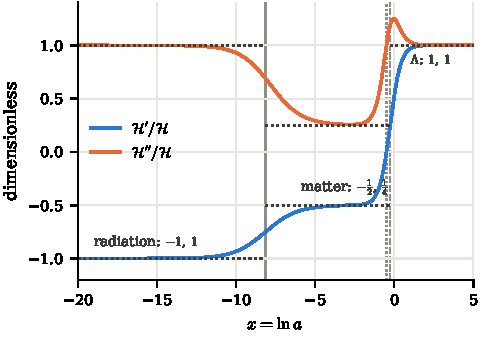
\includegraphics[width=\columnwidth]{m1_Hp_derivatives}
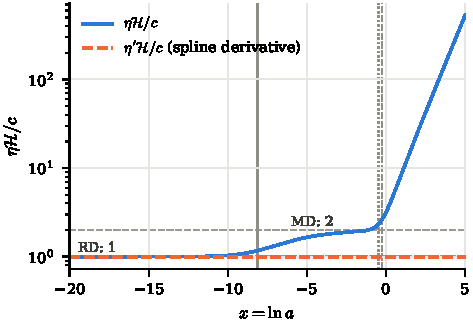
\includegraphics[width=\columnwidth]{m1_etaHp}
\caption{Tests of the background. \emph{Top:} $\Hp'/\Hp$ and $\Hp''/\Hp$. The short dotted lines are the analytic
values of Eq.~\eqref{eq:Hp_limits} in the radiation, matter and $\Lambda$ eras. \emph{Bottom:} $\eta\Hp/c$, which is
1 in RD and approaches 2 in MD, and $\eta'\Hp/c$ from the derivative of the spline, which should be exactly 1. In all
Milestone~I figures the vertical lines mark radiation--matter equality (solid), matter--$\Lambda$ equality (dashed) and
the onset of acceleration (dotted).}
\label{fig:Hp_tests}
\end{figure}

\subsection{Results}

The expansion history is shown in Figs.~\ref{fig:Hp}--\ref{fig:Omegas} and the key epochs are listed in
Table~\ref{tab:m1}.

\paragraph*{The three eras.} Figure~\ref{fig:Omegas} shows the succession of eras that follows from the different
dilution laws. Going back in time, radiation ($\propto a^{-4}$) eventually wins over matter ($\propto a^{-3}$), which
in turn wins over the constant $\rho_\Lambda$. Radiation dominates until $z=3400$, when the Universe was only
$51\,000$ years old. Matter then dominates for most of cosmic history, and $\Lambda$ only takes over at $z=0.29$. Before
$z\sim2$ the cosmological constant is completely negligible; that we happen to live just when $\Om_M$ and $\Om_\Lambda$
are comparable is the so-called coincidence problem. Today $\Om_{\Lambda0}=0.6829$, $\Om_{\gamma0}=5.51\times10^{-5}$
and $\Om_{\nu0}=3.81\times10^{-5}$.

\paragraph*{The conformal Hubble factor.} $\Hp$ (Fig.~\ref{fig:Hp}) falls as $e^{-x}$ in RD and as $e^{-x/2}$ in MD,
exactly as Eq.~\eqref{eq:Hp_limits} predicts. Because $\Hp=\dot a$, its slope is the sign of the acceleration: $\Hp$
has a minimum exactly at the onset of acceleration, $z=0.627$, and then grows as $e^{x}$. Acceleration starts well
before matter--$\Lambda$ equality at $z=0.292$, because the pressure of the cosmological constant counts twice in
Eq.~\eqref{eq:accel}: $\Lambda$ only needs half the matter density to make $\ddot a>0$. A falling $\Hp$ means the
comoving Hubble radius $c/\Hp$ grows and new scales enter the horizon; after $z=0.63$ this has reversed, and scales
are now leaving the horizon again.

\paragraph*{Age and horizon.} The age of the Universe is $t_0=13.85$\,Gyr (Fig.~\ref{fig:times}). This is
$0.949\,H_0^{-1}$, with $H_0^{-1}=14.59$\,Gyr. A flat matter-only (Einstein--de Sitter) universe with the same $H_0$
would be only $\tfrac23H_0^{-1}=9.7$\,Gyr old, younger than the oldest stars. The cosmological constant slowed the
expansion less in the past, so it took longer to reach today's expansion rate, and the Universe is older. The
conformal time today is $\eta_0/c=46.29$\,Gyr ($\eta_0=14\,192\Mpc=3.17\,c/H_0$). This is the comoving radius of the
observable Universe: light has travelled for 13.85\,Gyr, but the space it crossed has expanded in the meantime.

The radiation era is short in cosmic time but long in conformal time, because $\dd\eta=c\,\dd t/a$ weighs early times
by $1/a$. About $40\%$ of the conformal time at recombination accumulates before equality. The comoving horizon at
recombination is $\eta_*\approx280\Mpc$, only $2\%$ of the distance $\eta_0-\eta_*$ to the last-scattering surface. It
subtends an angle of about $1^\circ$ on the sky. Regions of the CMB separated by more than this were causally
disconnected at recombination, which is the horizon problem that inflation is invoked to solve. It is also why the
acoustic features of the CMB appear at $\ell\sim200$ (Sec.~\ref{sec:m4}).

\begin{table}
\caption{Key epochs of the fiducial background. The ages are cosmic times since the Big Bang.}
\label{tab:m1}
\begin{ruledtabular}
\begin{tabular}{lccc}
Event & $x$ & $z$ & $t$ \\
\hline
Radiation--matter equality & $-8.1319$ & $3400.3$ & $51\,029$\,yr \\
Onset of acceleration       & $-0.4865$ & $0.6267$ & $7.750$\,Gyr \\
Matter--$\Lambda$ equality  & $-0.2558$ & $0.2915$ & $10.371$\,Gyr \\
Today                       & $0$       & $0$      & $13.848$\,Gyr \\
\end{tabular}
\end{ruledtabular}
\end{table}

\begin{figure}
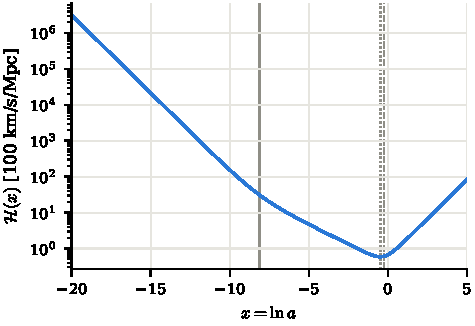
\includegraphics[width=\columnwidth]{m1_Hp}
\caption{The conformal Hubble factor $\Hp=aH=\dot a$ in units of $100$\,km\,s$^{-1}$\,Mpc$^{-1}$. It decreases during
RD and MD, when the expansion decelerates, and increases after the onset of acceleration (dotted line).}
\label{fig:Hp}
\end{figure}

\begin{figure}
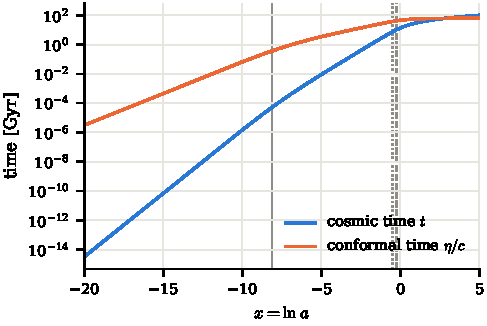
\includegraphics[width=\columnwidth]{m1_times}
\caption{Cosmic time $t$ and conformal time $\eta/c$ in Gyr. In RD $t\propto a^2$ and $\eta\propto a$; in MD
$t\propto a^{3/2}$ and $\eta\propto a^{1/2}$. $\eta$ freezes at $\eta_0/c=46.3$\,Gyr in the $\Lambda$ era, while $t$
grows logarithmically in $a$.}
\label{fig:times}
\end{figure}

\begin{figure}
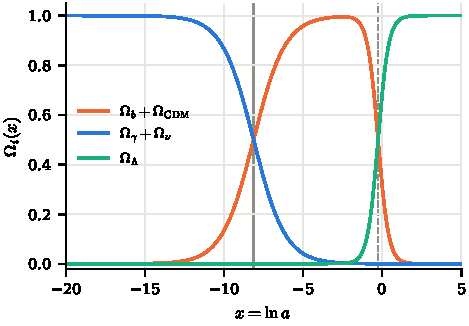
\includegraphics[width=\columnwidth]{m1_Omegas}
\caption{Density parameters of relativistic species ($\Om_\gamma+\Om_\nu$), matter ($\Om_b+\Om_{\rm CDM}$) and dark
energy ($\Om_\Lambda$) as functions of $x$. They always sum to one in a flat universe.}
\label{fig:Omegas}
\end{figure}

\paragraph*{Supernovae.} Type Ia supernovae are standardizable candles: after empirical corrections for light-curve
width and colour, their peak luminosities are nearly the same. Their fluxes therefore measure $d_L(z)$.
Figure~\ref{fig:sn} compares our luminosity distance with the binned JLA distances of Betoule et
al.~\cite{Betoule2014}, plotted as $d_L/z$. At low redshift $d_L/z\to c/H_0$, and the rise with $z$ measures
$1-q_0$. Our model has $q_0=-0.52$.

The fiducial model reproduces the shape of $d_L(z)$ but is about $4\%$ too far away at all redshifts, giving
$\chi^2=141.7$ for $N=31$ points. With the density parameters fixed, $d_L\propto1/h$ and $h$ only rescales the curve.
The best fit is then $h=0.699$ with $\chi^2=30.7$, a good fit. The data clearly require acceleration. For comparison,
the best fit of a flat matter-only universe (EdS, $q_0=+\frac12$) gives $\chi^2=317$, and even an empty, coasting
universe ($q_0=0$) gives $\chi^2=49$.

The preference for $h\approx0.70$ should not be read as a measurement of $H_0$. Supernovae measure \emph{relative}
distances. The absolute scale of the data comes from the absolute magnitude adopted when converting the distance
moduli to $d_L$, which is degenerate with $H_0$. A joint fit of $h$, $\Om_{M0}$ and $\Om_{K0}$ by MCMC is part of the
course project but omitted here.

\begin{figure}
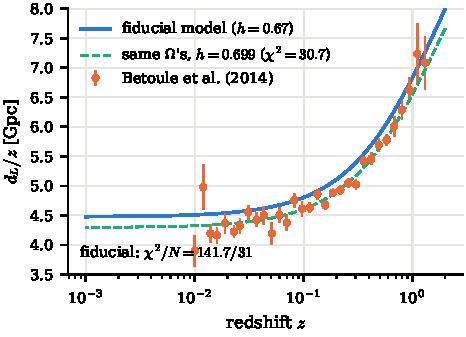
\includegraphics[width=\columnwidth]{m1_supernovae}
\caption{Luminosity distance divided by redshift for the fiducial model (solid), and for the same density parameters
with the best-fit $h$ (dashed), compared with the binned JLA supernova data~\cite{Betoule2014}. The intercept at $z\to0$
is $c/H_0$; the slope measures the acceleration of the expansion.}
\label{fig:sn}
\end{figure}
